\section{Evklidske in origami konstrukcije}

Kraj in čas izvora origamija nista jasno določena. Nekateri viri zatrjujejo, da izhaja iz Japonske, drugi ga pripisujejo Kitajski, tretji se ne strinjajo z nobeno od teh dveh možnosti. Možno je, da so umetnost zlaganja odkrili še pred izumom papirja, za katerega je l. 105 po Kr. poskrbel kitajski dvorni uradnik Cai Lun, saj se da npr.\ zlagati tudi robce iz blaga. Je pa papir idealen material za zlaganje. Japonska beseda \emph{origami} kot umetnost zgibanja papirja (``oru'' -- prepogibati, ``kami'' -- papir) se je na Daljnem vzhodu začela uporabljati proti koncu 19. stoletja.

Povečano zanimanje za origami v matematiki se je začelo v 2.\ pol.\ 20.\ stoletja in s seboj prineslo množično izhajanje literature o povezavi origamija z matematiko, fiziko, astronomijo, računalništvom, kemijo in še mnogimi drugimi vedami~\cite{zore2022}. V angleščini je tako za matematično raziskovanje s prepogibanjem papirja nastal izraz ``\emph{origamics}'', ki bi ga lahko po zgledu poimenovanj veliko znanstvenih disciplin (\emph{mathematics} -- matematika, \emph{physisc} -- fizika itd.) prevedli kot ``origamika''~\cite{sgv2016} (uradnega izraza v slovenščini še ni).

\subsection{Evklidovi postulati in evklidske konstrukcije}

Preden si pogledamo, kaj lahko s prepogibanjem papirja konstruiramo, se spomnimo, na čem temelji evklidska geometrija. Za njenega očeta štejemo grškega matematika Evklida\footnote{O življenju tega aleksandrijskega učenjaka ne vemo nič gotovega, je pa zelo verjetno živel za časa prvega Ptolemaja (faraon v času 306--283 pr.\ Kr.)~\cite[str.\ 61]{struik1986}.}, ki je napisal zelo znano zbirko trinajstih knjig pod skupnim imenom \emph{Elementi}. V njih obravnavana snov temelji na strogo logični izpeljavi izrekov iz definicij\footnote{\emph{Definicija} je nedvoumno jasna opredelitev novega pojma.}, aksiomov\footnote{\emph{Aksiom} je temeljna resnica ali načelo, ki ne potrebuje dokazov (oz.\ dokaz sploh ne obstaja) in vedno velja.} in postulatov\footnote{\emph{Postulat} je predpostavka oz.\ zahteva. Evklid med aksiomi in postulati ni postavil jasne razlike, Aristotel pa je postulat od aksioma ločil po tem, da gre pri prvem bolj za hipotezo kot temeljno resnico, vendar se njene veljavnosti ne dokazuje, temveč privzame kot veljavno~\cite[str.\ 122]{euclidI}. V primeru petega Evklidovega postulata se bomo spomnili, da nam to, ali ga privzamemo ali ne, poda različne geometrije. Danes med pojmoma ne ločujemo~\cite[str.\ 2]{geometricconstructions}.}. Še danes večina osnovno- in srednješolske geometrije izvira prav iz prvih šestih knjig Elementov.

Prva knjiga nas še posebej zanima. V njej je Evklid najprej definiral osnovne pojme -- točka, premica, površina, ravnina, ravninski kot, pravi kot, ostri kot, topi kot, krog, središče kroga, premer, enakostranični in enakokraki trikotnik, kvadrat \ldots ter nazadnje upeljal še pojem vzporednih premic. Nato je zapisal znamenitih pet postulatov~\cite{euclidI}, iz katerih izhaja vsa evklidska geometrija:

\renewcommand{\thepostulat}{P\arabic{postulat}}

\begin{postulat}
    \label{post:P1}
    Med dvema poljubnima točkama je mogoče narisati ravno črto.
\end{postulat}
\begin{postulat}
    \label{post:P2}
    Vsako ravno črto je mogoče na obeh koncih podaljšati.
\end{postulat}
\begin{postulat}
    \label{post:P3}
    Mogoče je narisati krožnico s poljubnim središčem in poljubnim polmerom.
\end{postulat}
\begin{postulat}
    \label{post:P4}
    Vsi pravi koti so med seboj skladni.
\end{postulat}
\begin{postulat}
    \label{post:P5}
    Če poljubni ravni črti sekamo s tretjo ravno črto (prečnico) in je vsota notranjih kotov eni strani prečnice manjša od dveh pravih kotov, potem se dani premici, če ju dovolj podaljšamo, sekata na tej strani prečnice.
    \opomba{Vemo že, da je postulat~\ref{post:P5} ekvivalenten \emph{aksiomu o vzporednicah}, ki pravi, da skozi dano točko, ki ne leži na dani premici, poteka natanko ena vzporednica k tej premici.}
\end{postulat}

\emph{Evklidske konstrukcije} so konstrukcije premic, kotov, krožnic in drugih geometrijskih figur, ki jih je mogoče konstruirati le z uporabo t.\i.\ \emph{evklidskih orodij}:

\begin{itemize}
    \item neoznačeno in neskončno dolgo ravnilo (angl.\ \emph{straightedge})
    \item šestilo, ki ne prenaša razdalj (ko ga dvignemo od podlage, se njegova kraka zložita skupaj)
\end{itemize}

Formalno so torej edine dovoljene konstrukcije tiste iz postulatov~\ref{post:P1}--~\ref{post:P3} (seveda privzamemo, da so konstruktibilne tudi točke). Vendar je to dovolj, da lahko le z neoznačenim ravnilom in šestilom konstruiramo premice, kote, simetrale kotov in daljic, krožnice in še mnogo drugega. V resnici se da skonstruirati toliko geometrijskih figur, da se matematiki raje vprašamo, česa pa se s tem orodjem \emph{ne} da skonstruirati. In tu pridemo do motivacije za uvedbo origami konstrukcij, saj lahko z njimi npr.\ rešimo kar dva od treh znamenitih starogrških problemov, ki jih z evklidskim orodjem ne moremo. Več o tem sledi v poglavju~\ref{pogl:starogrskiproblemi}.

\subsection{Origami aksiomi in origami konstrukcije}

V nalogi se bomo omejili le na prepogibanje v ravnini, tj.\ list papirja vzamemo za model evklidske ravnine, s prepogibanjem pa v tej ravnini tudi ostanemo. Nadalje pregibe konsktruiramo le po enega naenkrat in v ravni črti, prepovedana pa je uporaba kakršnegakoli orodja (npr.\ škarje in lepilo).  Bralec je ob branju povabljen, da opisane konstrukcije tudi sam preizkusi na listu papirja, sicer pa se jih da brez večjih težav predstavljati tudi brez fizičnega materiala.

Ker so pregibi torej ravne črte, nam služijo kot modeli premic. Na začetku, ko imamo pred seboj le (po možnosti kvadraten) list papirja, so naše premice njegove stranice. Manjkajo nam samo še modeli točk. To so ravno oglišča našega lista papirja, nadaljne točke pa dobimo kot presečišča premic, torej presečišča pregibov.

Japonski matematik Humiaki Huzita je l.\ 1992 (\textcolor{red}{REFERENCA 26 v uni knjigi, pa v bistvu ugotovi, kdo je original avtor in kdo je kasneje koliko aksiomov rediscoveral!}) zapisal seznam pravil, s katerimi lahko opišemo vse operacije, ki jih lahko naredimo s prepogibanjem papirja. \textcolor{red}{(najprej 6, pol 7, kako je to blo?????)} Konstrukcije, ki jih dobimo z upoštevanjem teh pravil, bomo poimenovali kar \emph{origami konstrukcije}. Ta pravila so znana pod imenom \textcolor{red}{\ldots} aksiomi, vendar je izbira izraza ``aksiom'' mogoče manj primerna, saj za nekatere od njih opisana konstrukcija ob neprimerno izbranih točkah in premicah sploh ne obstaja. Kljub temu bomo zaradi razširjenosti rabe to ime ohranili~\cite[str.\ 7]{zore2022}.

Najprej naštejmo te aksiome, potem pa si ob sledečih slikah poglejmo še prikaz opisanih konstrukcij. Videli bomo, da moramo pri nekaterih aksiomih ločiti več primerov~\cite{michael2005, zore2022}.

\renewcommand{\theaksiom}{O\arabic{aksiom}}

\begin{aksiom}
    \label{aks:O1}
    Za poljubni točki $A$ in $B$ obstaja natanko en pregib $p$, ki gre skoznju.
\end{aksiom}
\begin{aksiom}
    \label{aks:O2}
    Za poljubni točki $A$ in $B$ obstaja natanko en pregib $p$, da se točki pokrijeta.
\end{aksiom}
\begin{aksiom}
    \label{aks:O3}
    Za poljubni premici $a$ in $b$ obstaja pregib $p$, ki ju položi eno na drugo.
\end{aksiom}
\begin{aksiom}
    \label{aks:O4}
    Za poljubno točko $A$ in premico $a$ obstaja natanko en pregib $p$ skozi točko $A$, ki je pravokoten na premico $a$.
\end{aksiom}
\begin{aksiom}
    \label{aks:O5}
    Za primerno izbrani točki $A$ in $B$ ter premico $a$ obstaja pregib $p$ skozi točko $B$, ki točko $A$ postavi na premico $a$.
\end{aksiom}
\begin{aksiom}
    \label{aks:O6}
    Za primerno izbrani točki $A$ in $B$ ter premici $a$ in $b$ obstaja pregib $p$, ki točko $A$ postavi na premico $a$ ter točko $B$ na premico $b$.
\end{aksiom}

Sedaj za vsak aksiom posebej poglejmo njegovo konstrukcijo. Iz slike~\ref{fig:O1_in_O2} je očitno, da je aksiom~\ref{aks:O1} ekvivalenten postulatu~\ref{post:P1}, aksiom~\ref{aks:O2} pa nam poda konstrukcijo simetrale daljice $AB$ (pregib naredimo tako, da list papirja uvijemo tako, da se točki prekrijeta, nato pa ga z roko pogladimo, da ga sploščimo. Na pregibu -- premici -- so točke, ki so enako oddaljene od točk $A$ in $B$, torej gre res za simetralo daljice $AB$).

\begin{figure}[h!]
    \centering
    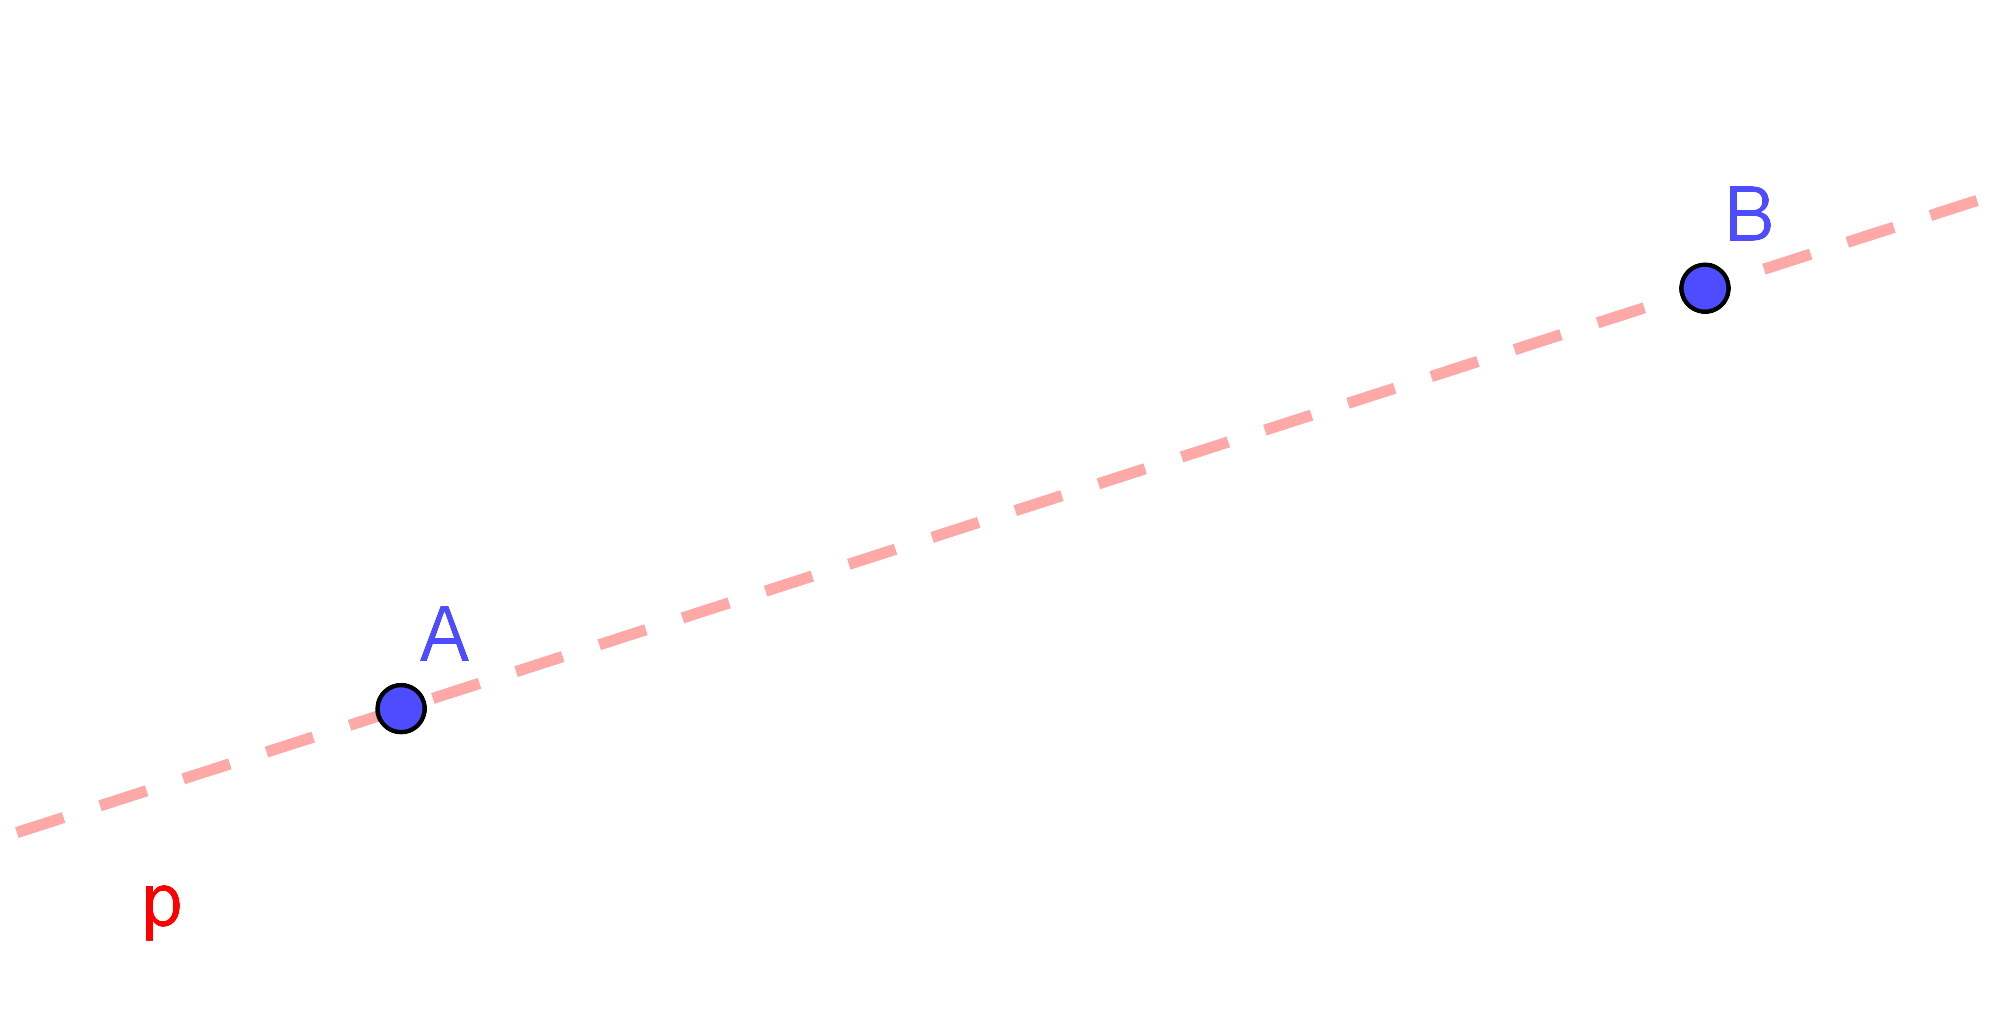
\includegraphics[width=0.5\textwidth]{images/origami_aksiomi/O1.png}
    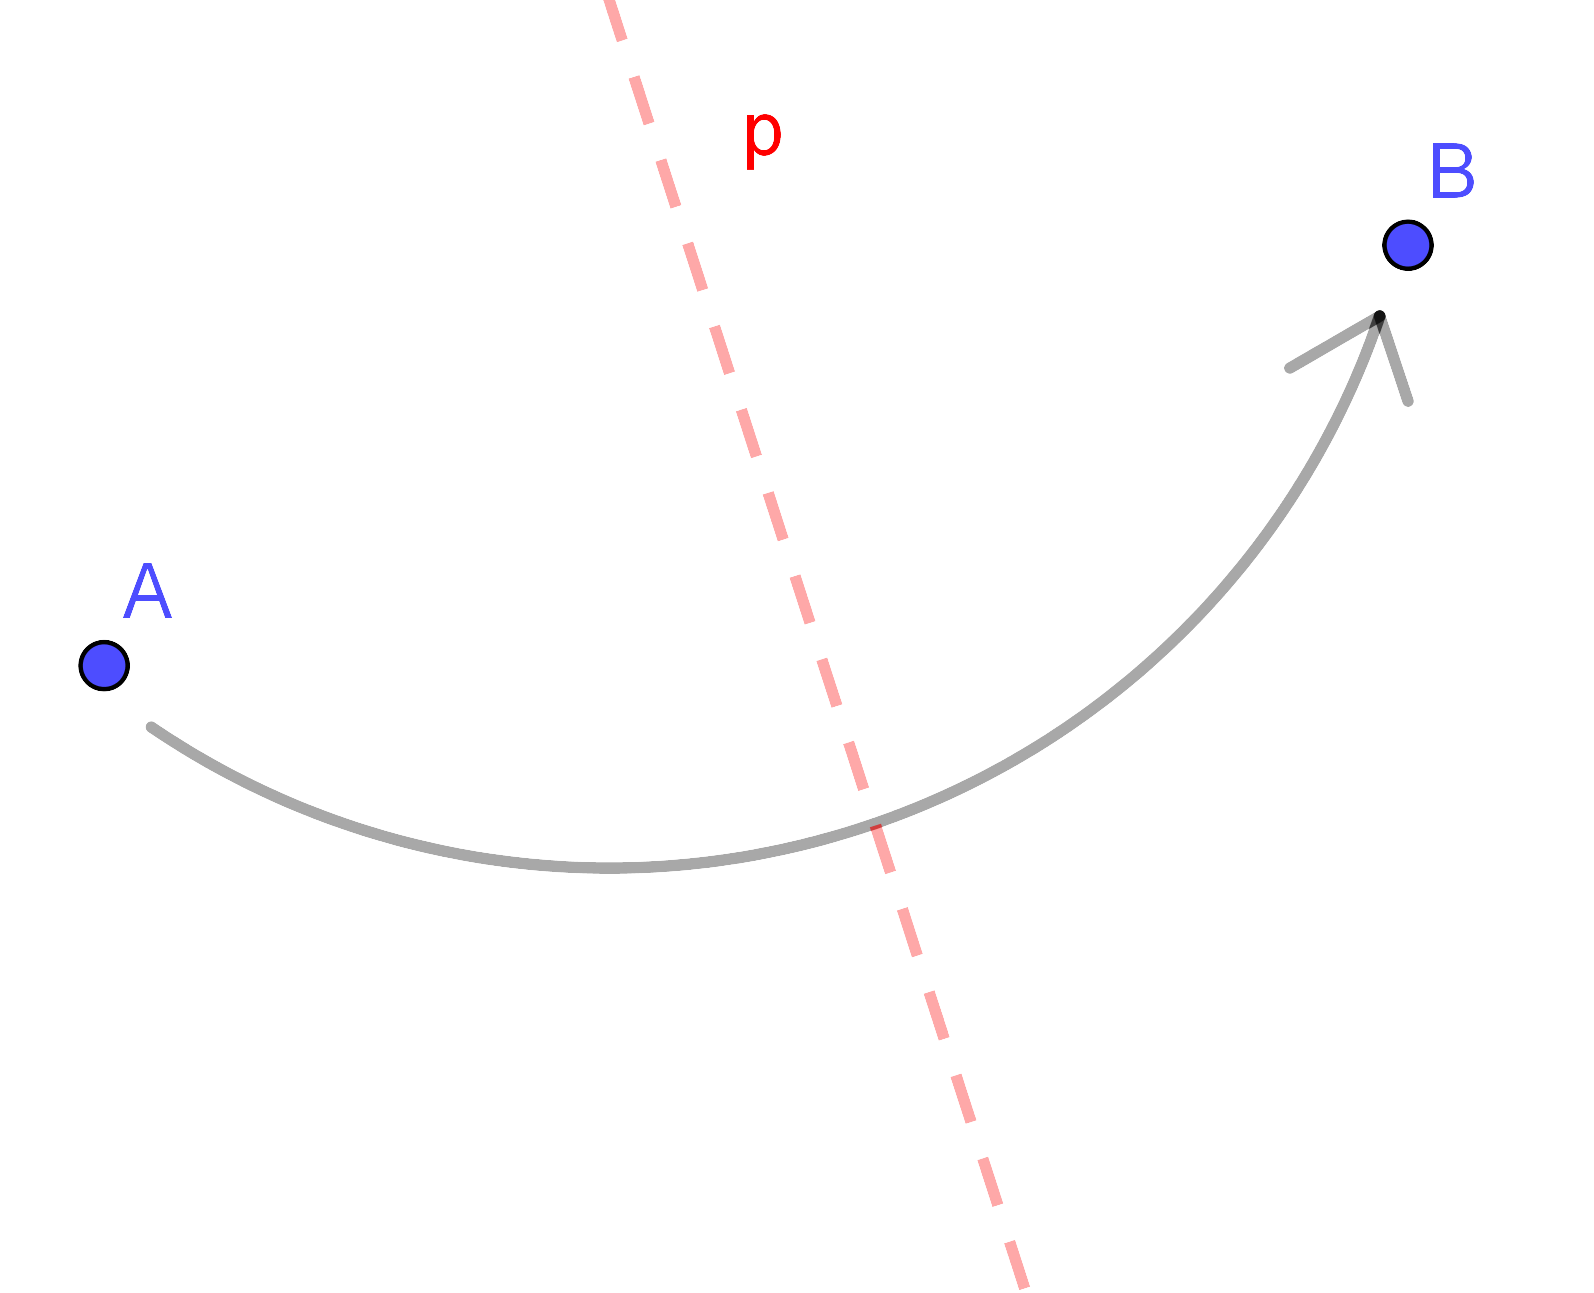
\includegraphics[width=0.4\textwidth]{images/origami_aksiomi/O2.png}
    \caption[Aksioma~\ref{aks:O1} in~\ref{aks:O2}]{Aksioma~\ref{aks:O1} (levo) in~\ref{aks:O2} (desno).}
    \label{fig:O1_in_O2}
\end{figure}

Nadalje opazimo, da nam aksiom~\ref{aks:O3} konstruira obe simetrali kota, ki ga določata premici in njuno presečišče, v primeru vzporednih premic pa dobimo še tretjo vzporednico, ki leži na sredi med njima (slika~\ref{fig:O3}). Zato sta tu možna po dva ali, v posebnem primeru, en pregib.

\begin{figure}[h!]
    \centering
    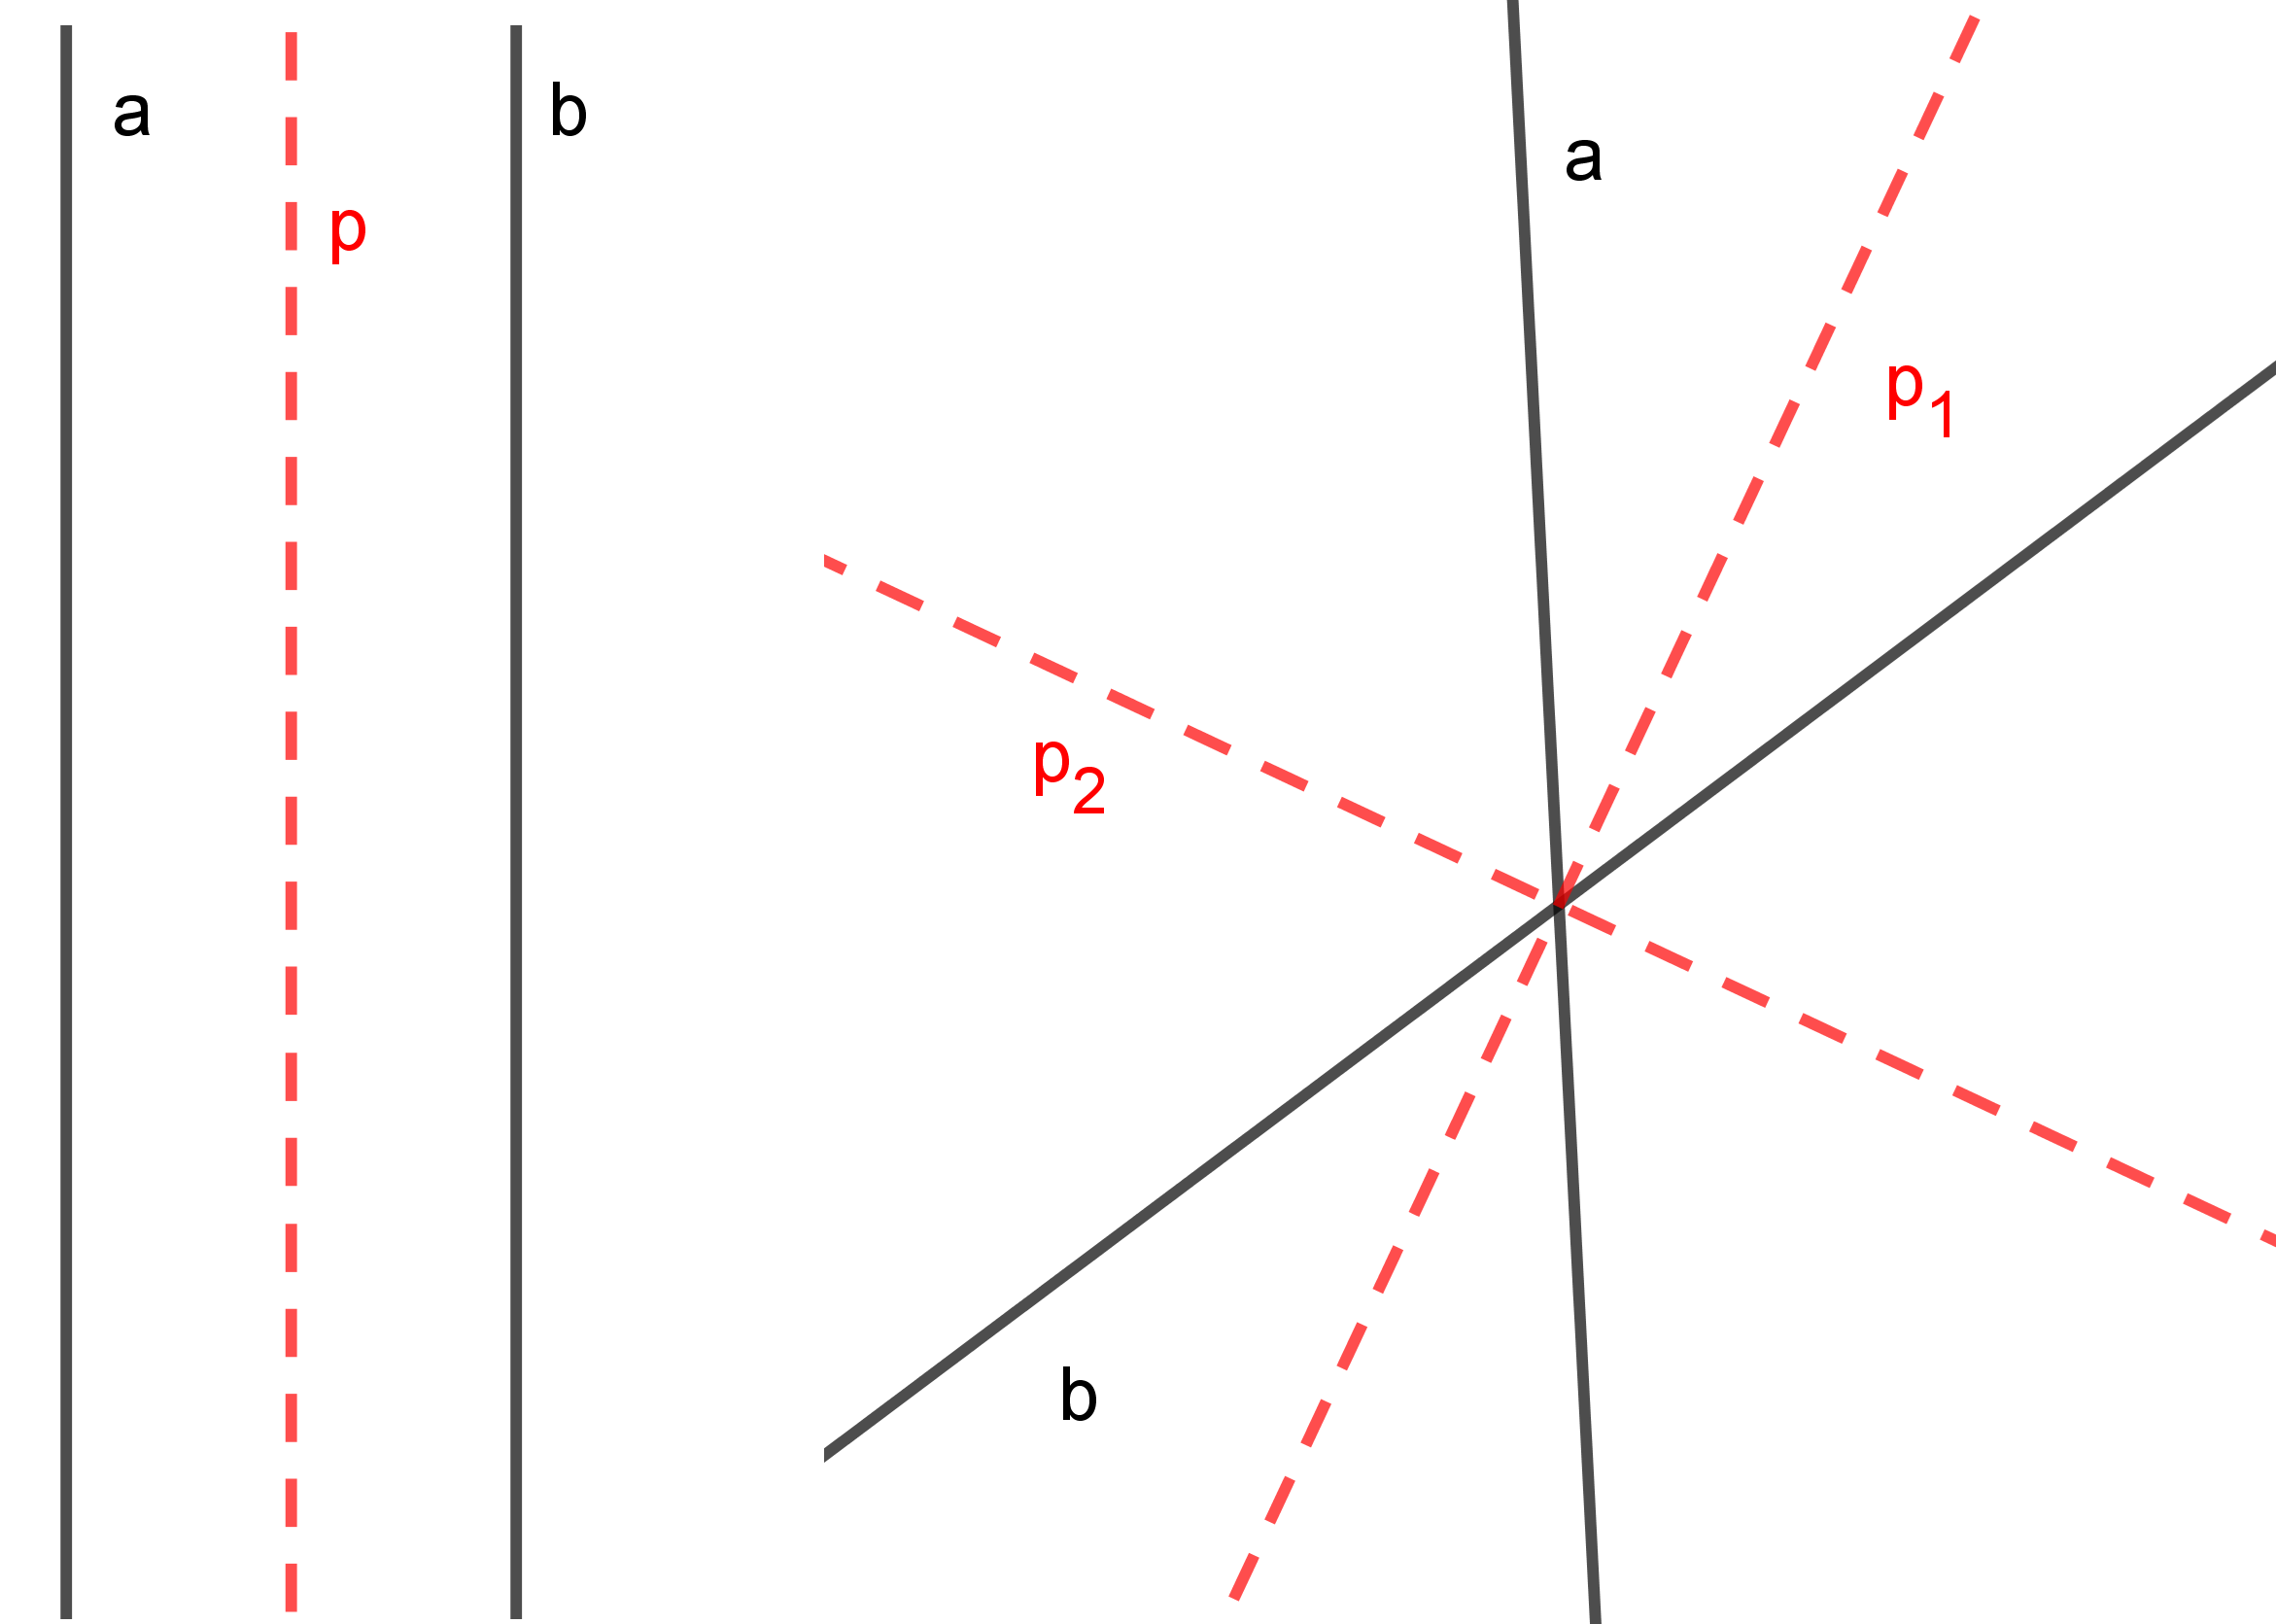
\includegraphics[width=0.5\textwidth]{images/origami_aksiomi/O3.png}
    \caption[Aksiom~\ref{aks:O3}]{Aksiom~\ref{aks:O3} v obeh možnih primerih.}
    \label{fig:O3}
\end{figure}

Aksiom~\ref{aks:O4} nam podaja konstrukcijo pravokotnice na premico skozi dano točko (slika~\ref{fig:O4}). Pri tem je vseeno, ali točka leži na premici ali ne. Pregib opravimo tako, da premico položimo samo nase in pazimo, da je točka $A$ v pregibu (ki ne more biti nič drugega kot pravokoten na premico). Tako imamo res le en možen pregib.

\begin{figure}[h!]
    \centering
    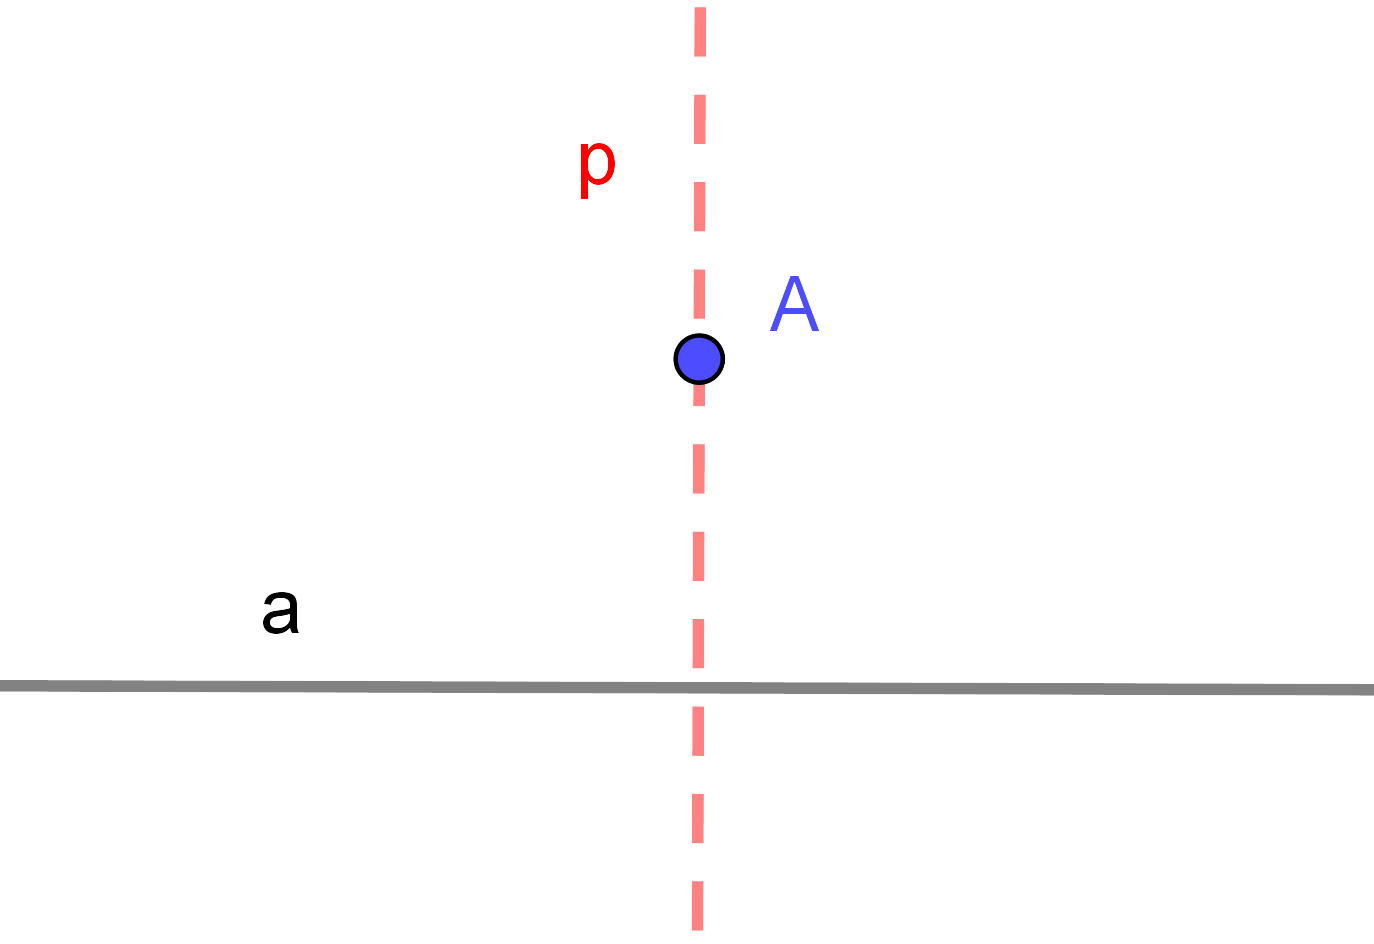
\includegraphics[width=0.4\textwidth]{images/origami_aksiomi/O4.png}
    \caption[Aksiom~\ref{aks:O4}]{Aksiom~\ref{aks:O4}.}
    \label{fig:O4}
\end{figure}

Aksiom~\ref{aks:O5} je še posebej zanimiv. Najprej si poglejmo njegovo konstrukcijo. Vzemimo točki $A$ in $B$ ter premico $a$. Iščemo pregib skozi $B$, ki $A$ položi na premico $a$. Ker točka $B$ leži na pregibu, je enako oddaljena tako od točke $A$ kot tudi njene slike $A'$ na premici $a$, torej je $A'$ ravno presečišče premice $a$ in krožnice s središčem v $B$ ter polmerom $AB$. Pregib je simetrala daljice $AA'$, seveda pa po konstrukciji poteka skozi točko $B$. Če velja $ d(A,B) > d(B,a) $, sta presečišči s premico $a$ dve (in s tem tudi dva možna pregiba), v primeru $ d(A,B) = d(B,a) $ je presečišče eno samo (in s tem en možen pregib), saj je premica $a$ tangentna na omenjeno krožnico, v zadnjem primeru, ko velja $ d(A,B) < d(B,a) $, pa presečišč (in s tem tudi pregiba) ni (slika~\ref{fig:O5}).

\begin{figure}[h!]
    \centering
    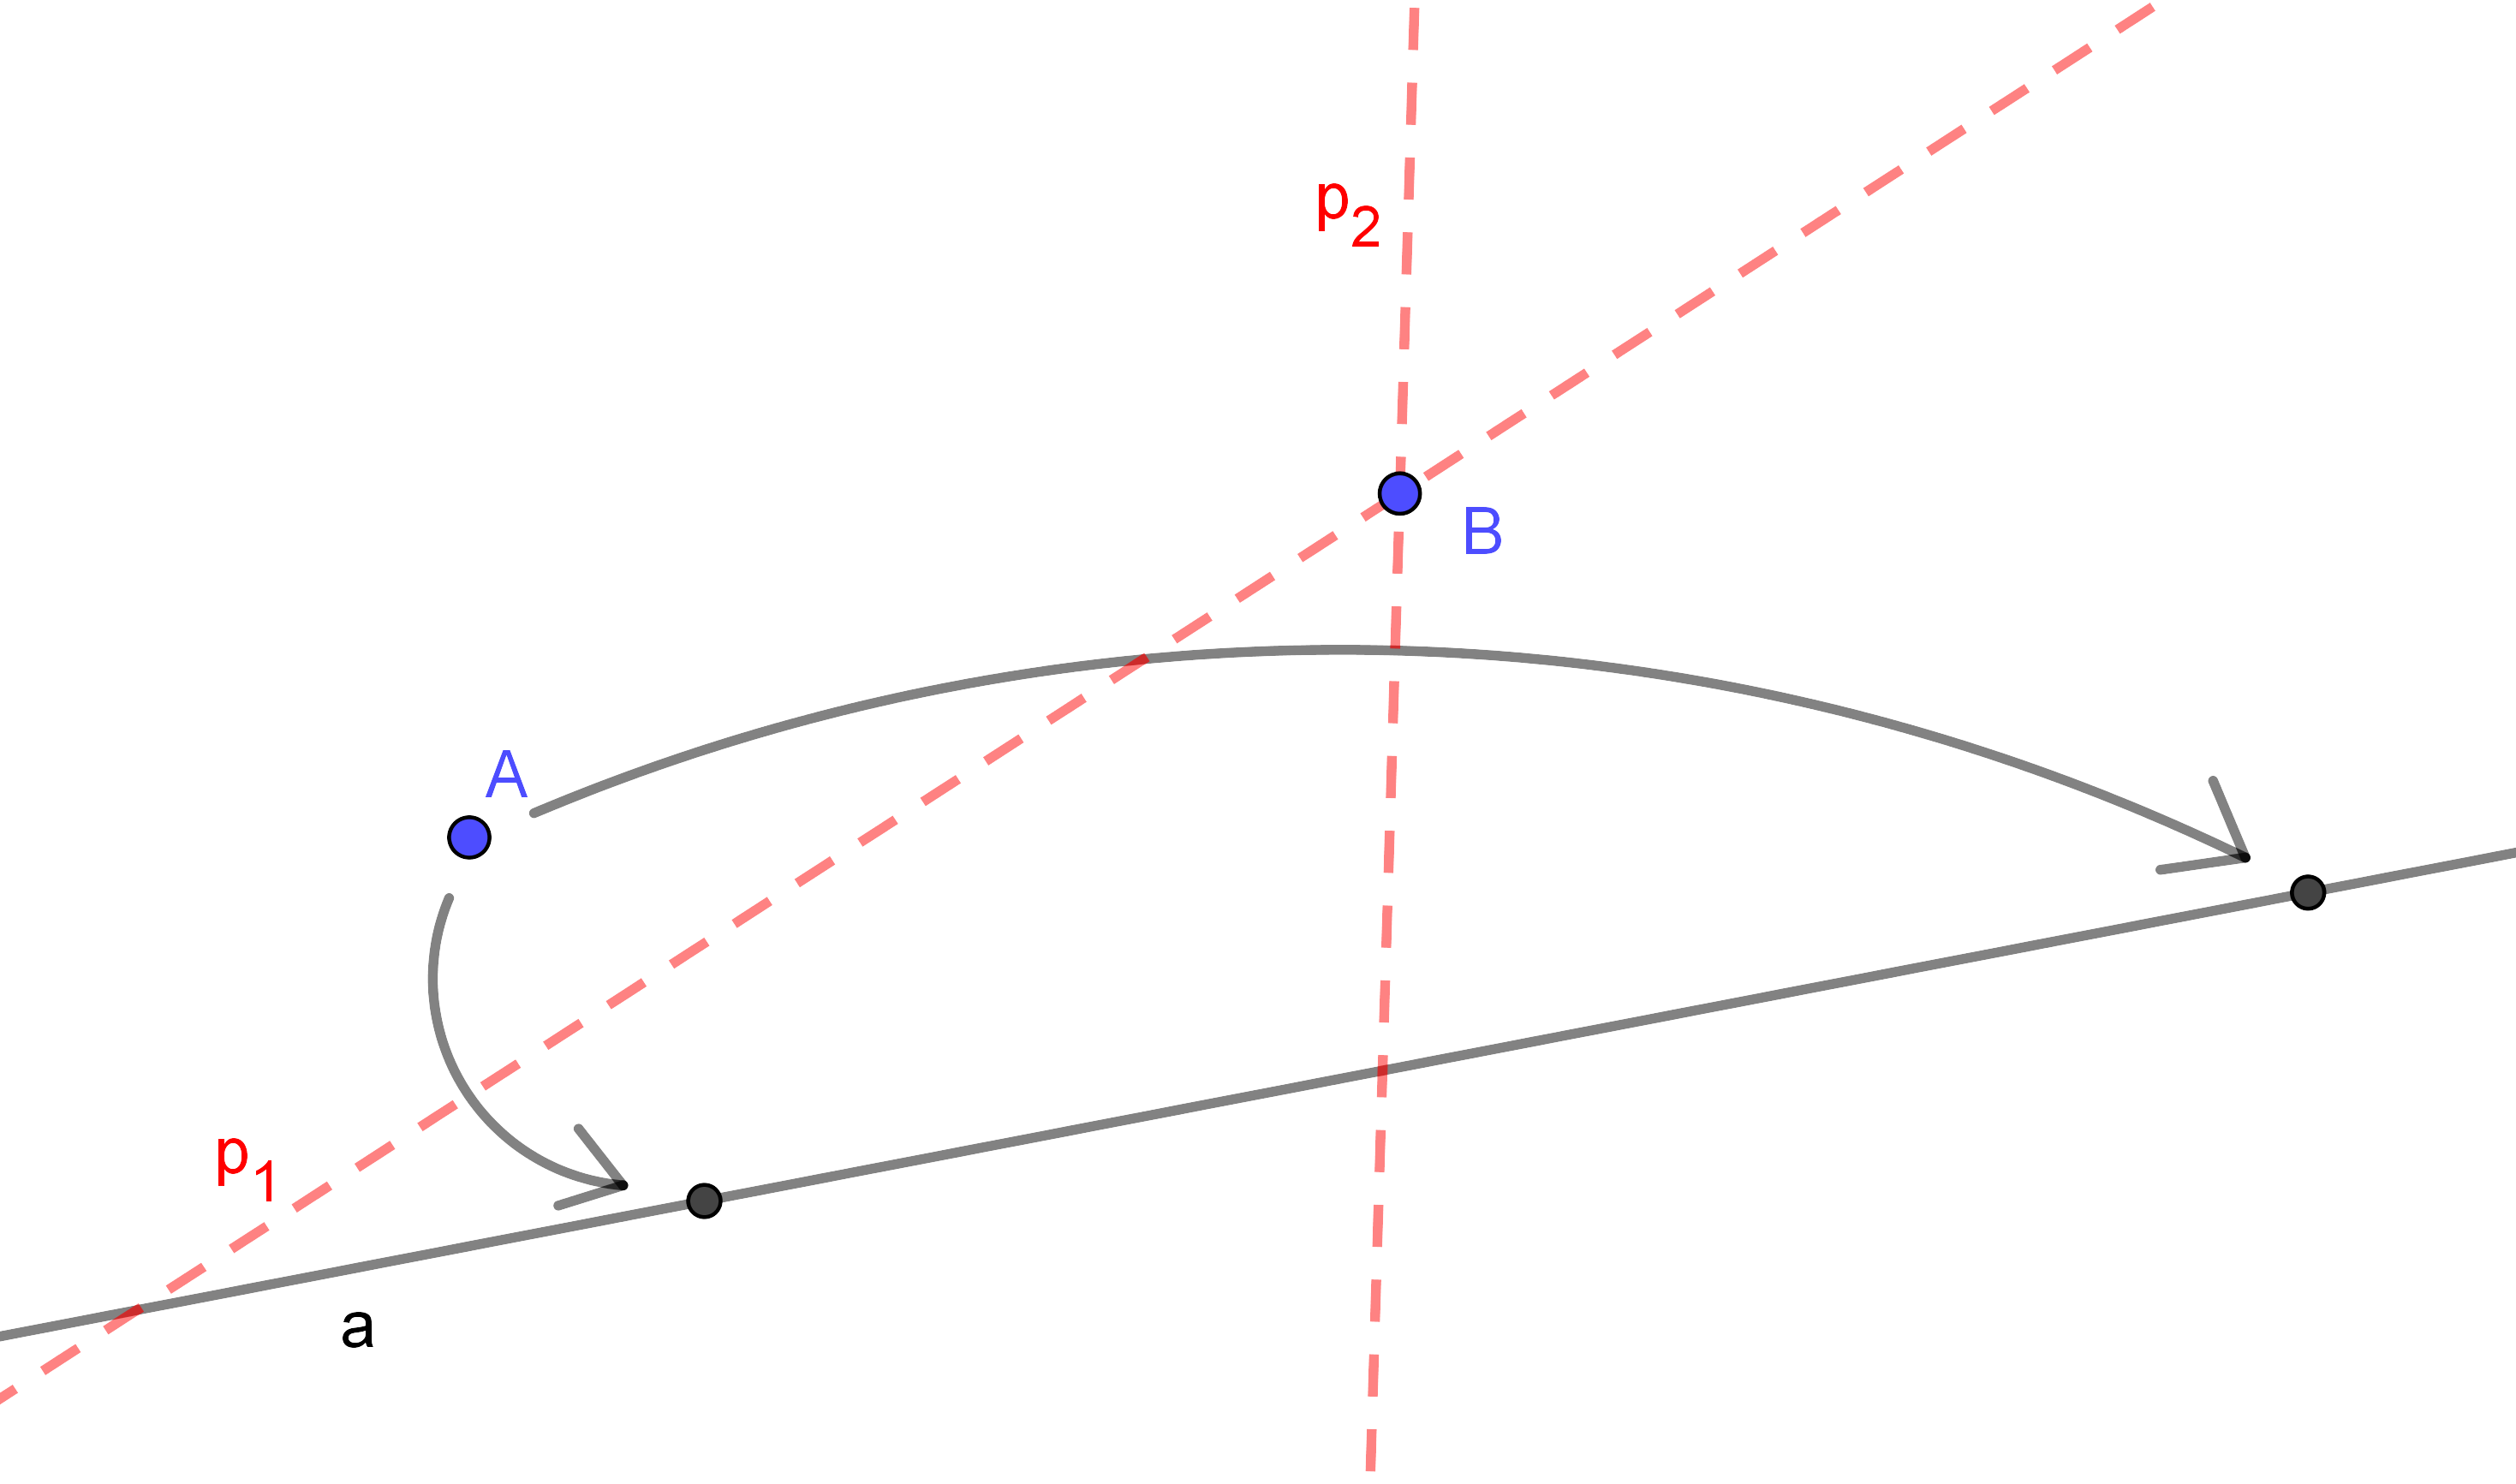
\includegraphics[width=0.55\textwidth]{images/origami_aksiomi/O5a.png}
    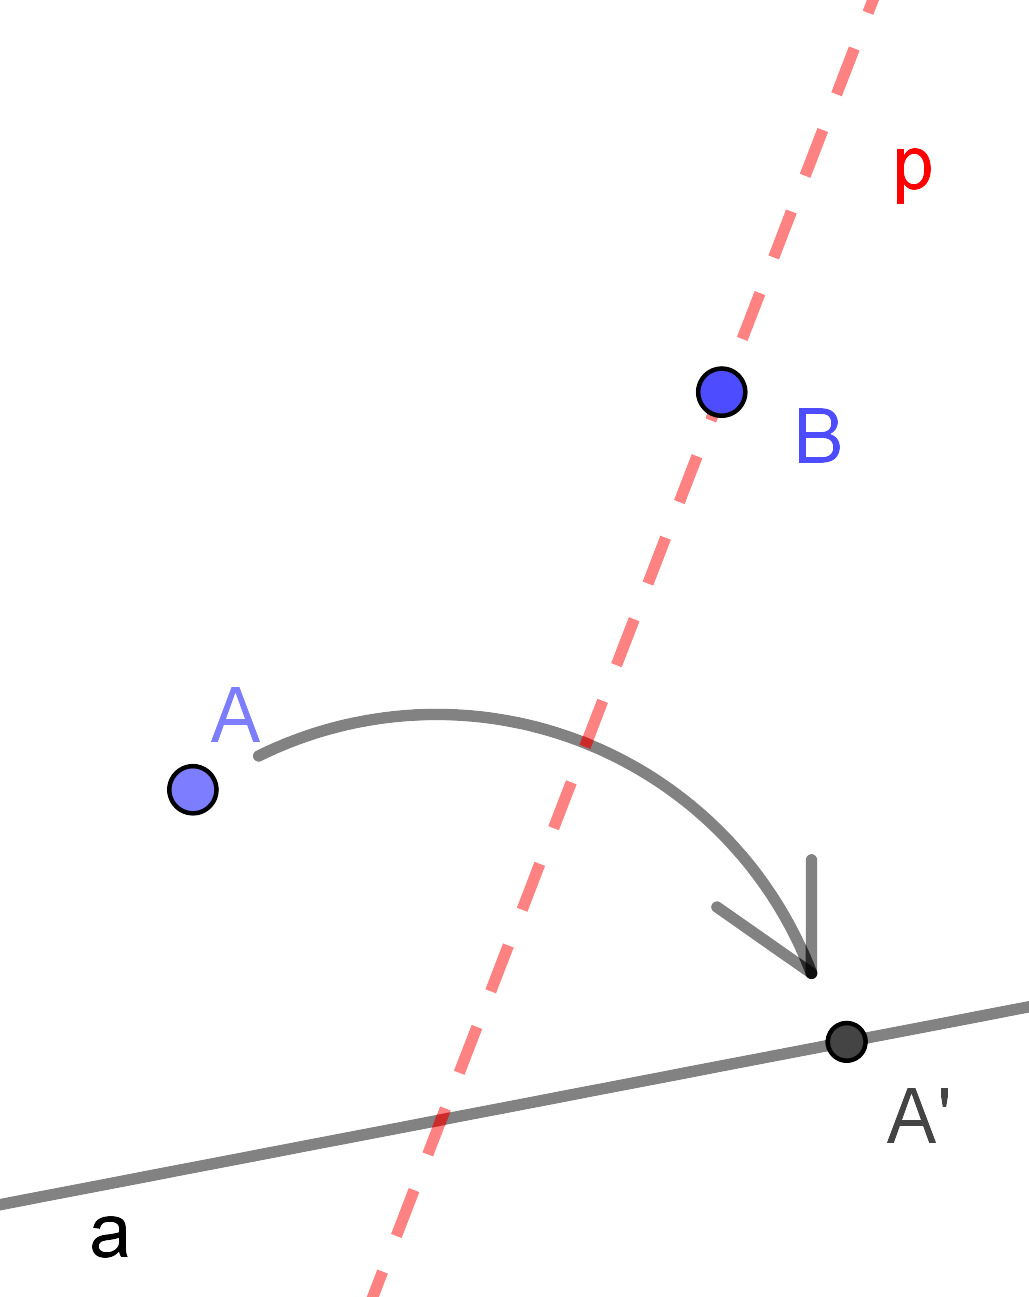
\includegraphics[width=0.2\textwidth]{images/origami_aksiomi/O5b.png}
    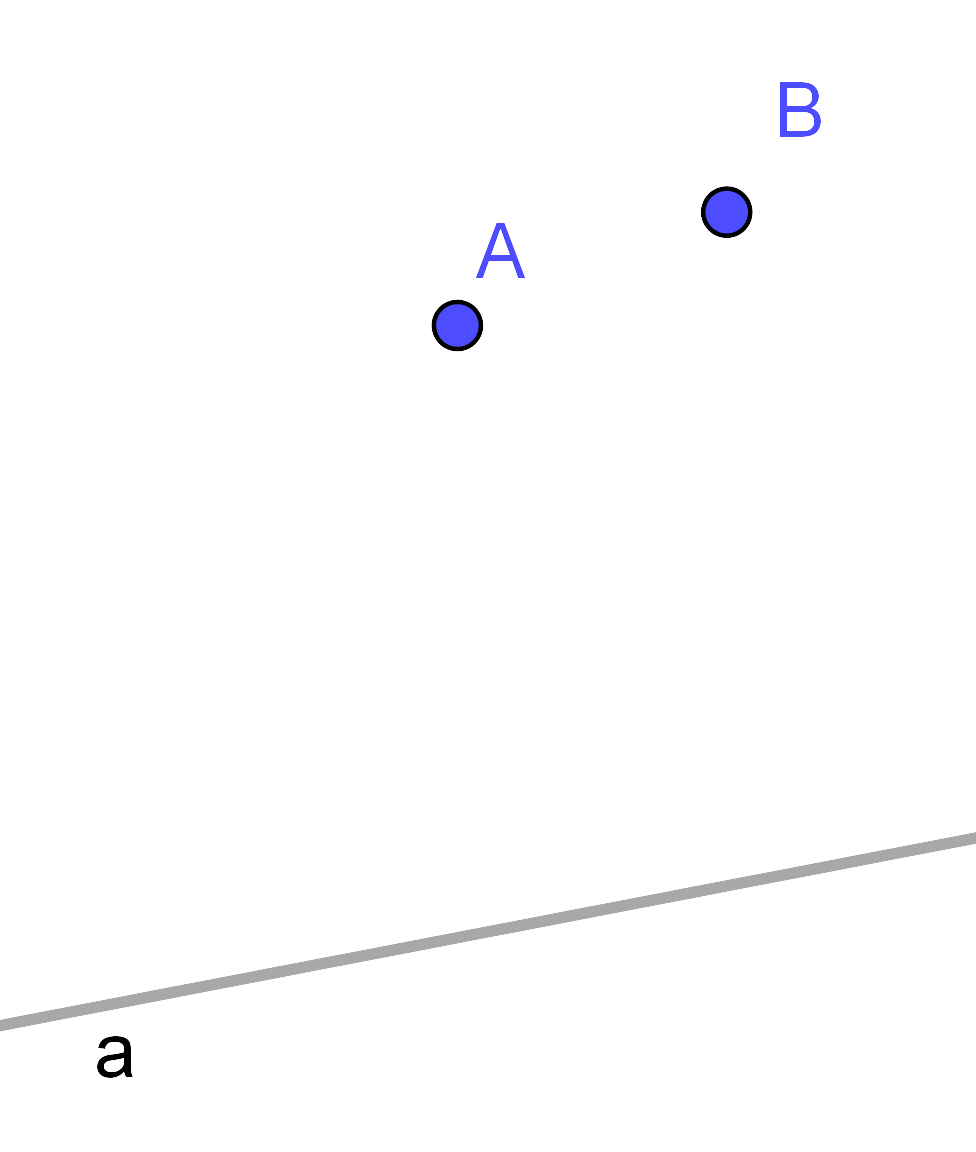
\includegraphics[width=0.2\textwidth]{images/origami_aksiomi/O5c.png}
    \caption[Aksiom~\ref{aks:O5}]{Aksiom~\ref{aks:O5} v vseh treh primerih.}
    \label{fig:O5}
\end{figure}

Zgodba aksioma~\ref{aks:O5} se tu še ne zaključi. Ker na pregibu ležijo vse točke, ki so enako oddaljene od točke $A$ in $A'$, to velja tudi za točko, ki jo dobimo kot presečišče pregiba in pravokotnice na premico $a$ skozi $A'$. Za tako točko $P$ velja $ d(A,P) = d(P,a) $ in je enolično določena (v srednjem primeru na sliki~\ref{aks:O5} je to kar točka $B$). Iz tega sledi, da točka $P$ leži na paraboli z goriščem $A$ in premico vodnico $a$. Pregib seka parabolo le v tej točki (ker je edina enako oddaljena od gorišče in vodnice), torej je konstruiran pregib ravno tangenta na to parabolo (slika~\ref{fig:O5_parabola}).

\begin{figure}[h!]
    \centering
    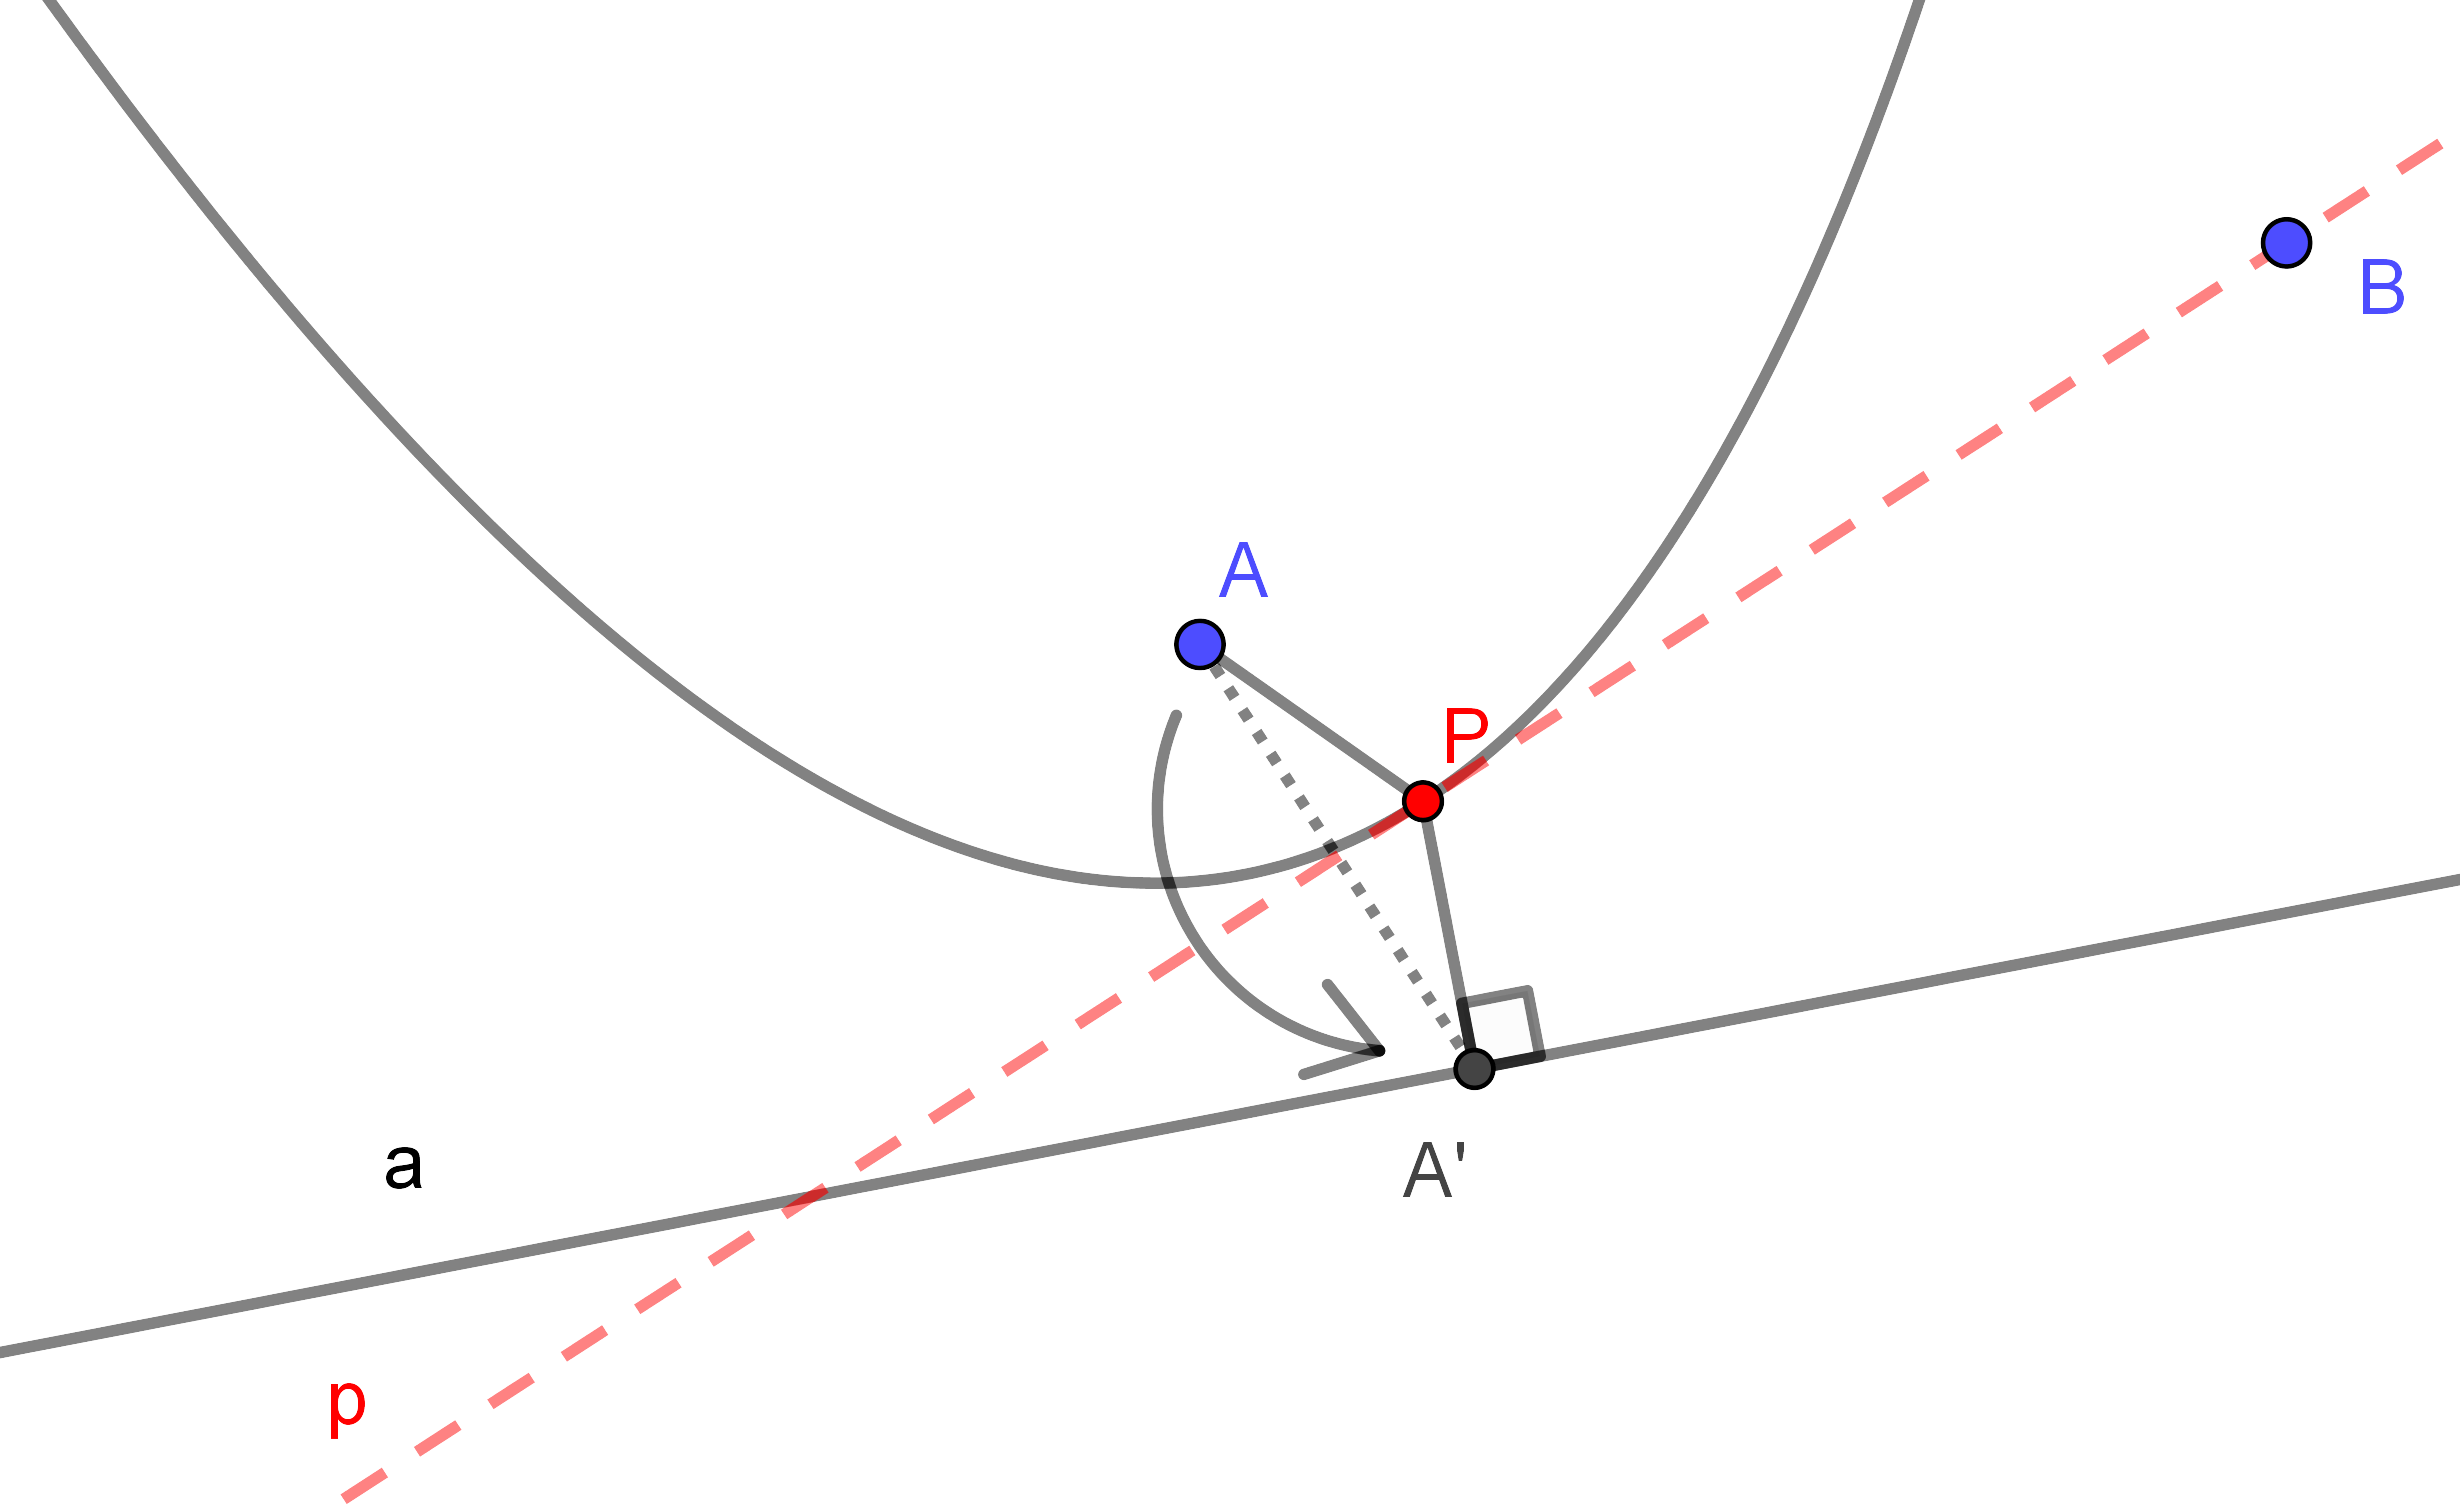
\includegraphics[width=0.6\textwidth]{images/origami_aksiomi/O5_parabola.png}
    \caption[Tangenta na parabolo]{Pregib iz aksioma~\ref{aks:O5} kot tangenta na parabolo z goriščem v $A$ in premico vodnico $a$.}
    \label{fig:O5_parabola}
\end{figure}

Opazimo, da se vse ravnokar naštete konstrukcije da konstruirati z evklidskim orodjem.

\textcolor{red}{DO TUKEJ}











\opomba{Za isto situacijo je lahko možnih več pregibov (gl.\ sliko~\ref{fig:O6}). Če sta premici vzporedni in je njuna medsebojna razdalja večja od razdalje med točkama, pa pregib ne obstaja. V poglavju~\ref{pogl:stoznice} bomo ta aksiom podrobneje preučili, saj nam podaja konstrukcijo skupne tangente na dve paraboli.}

\begin{figure}[h!]
    \centering
    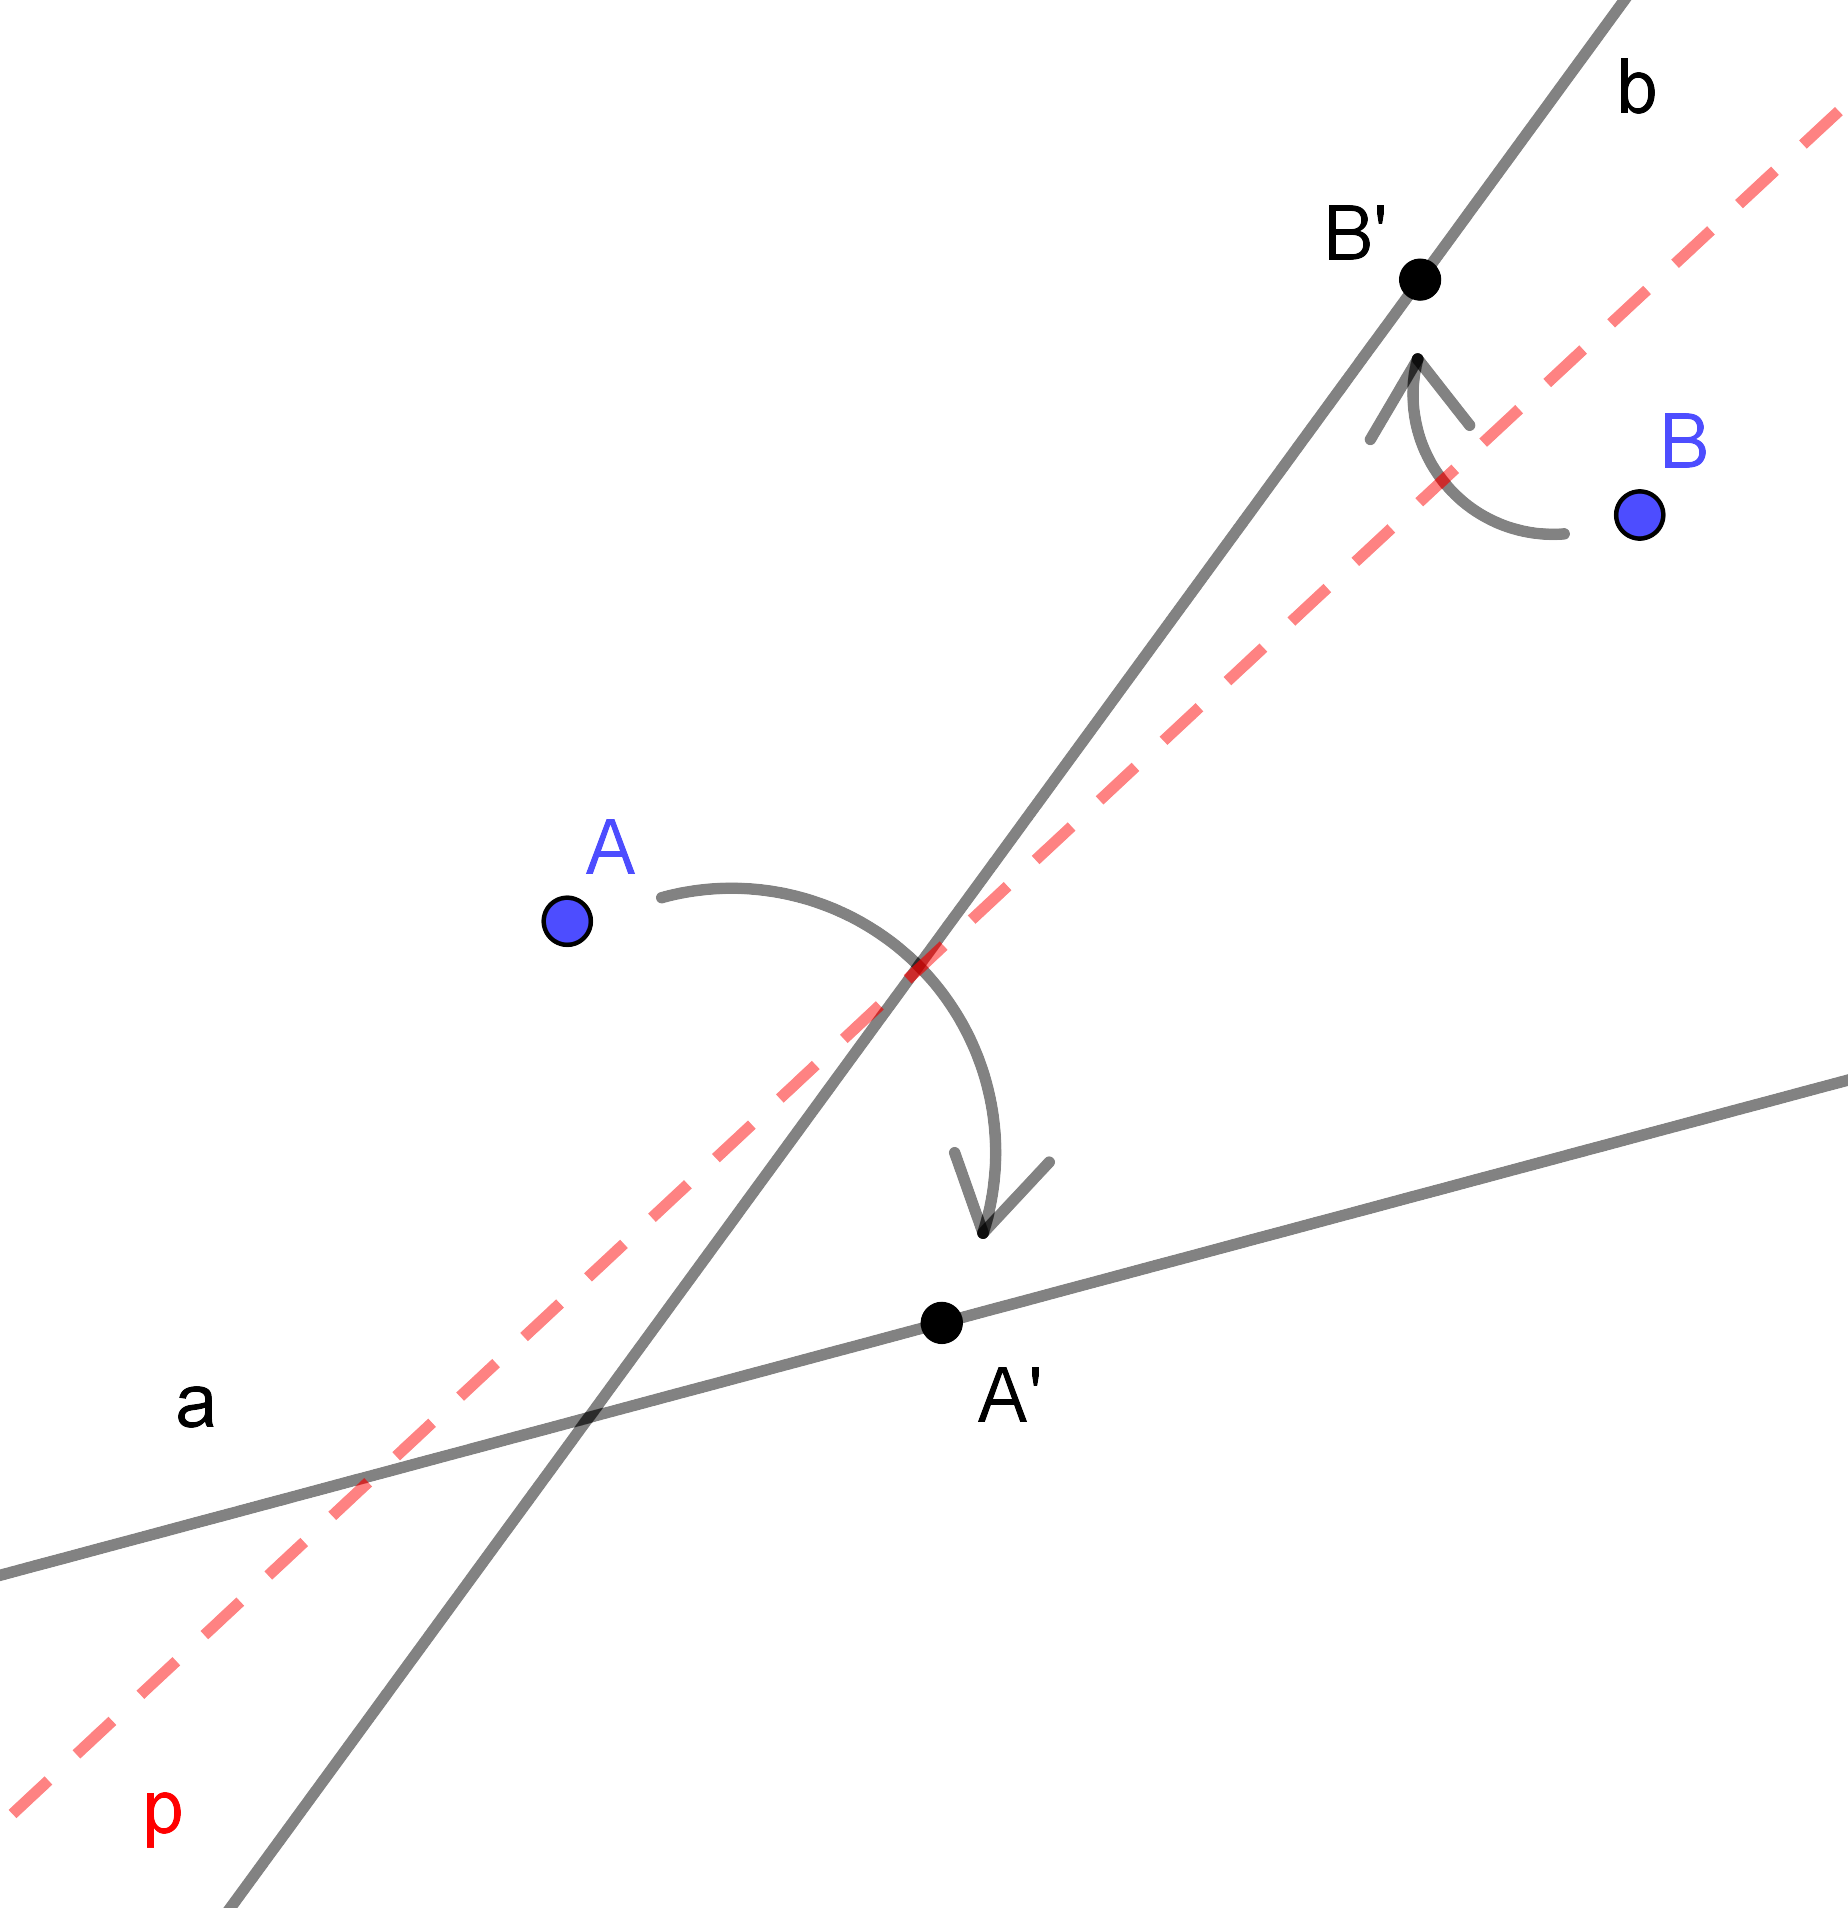
\includegraphics[width=0.45\textwidth]{images/origami_aksiomi/O6a.png}
    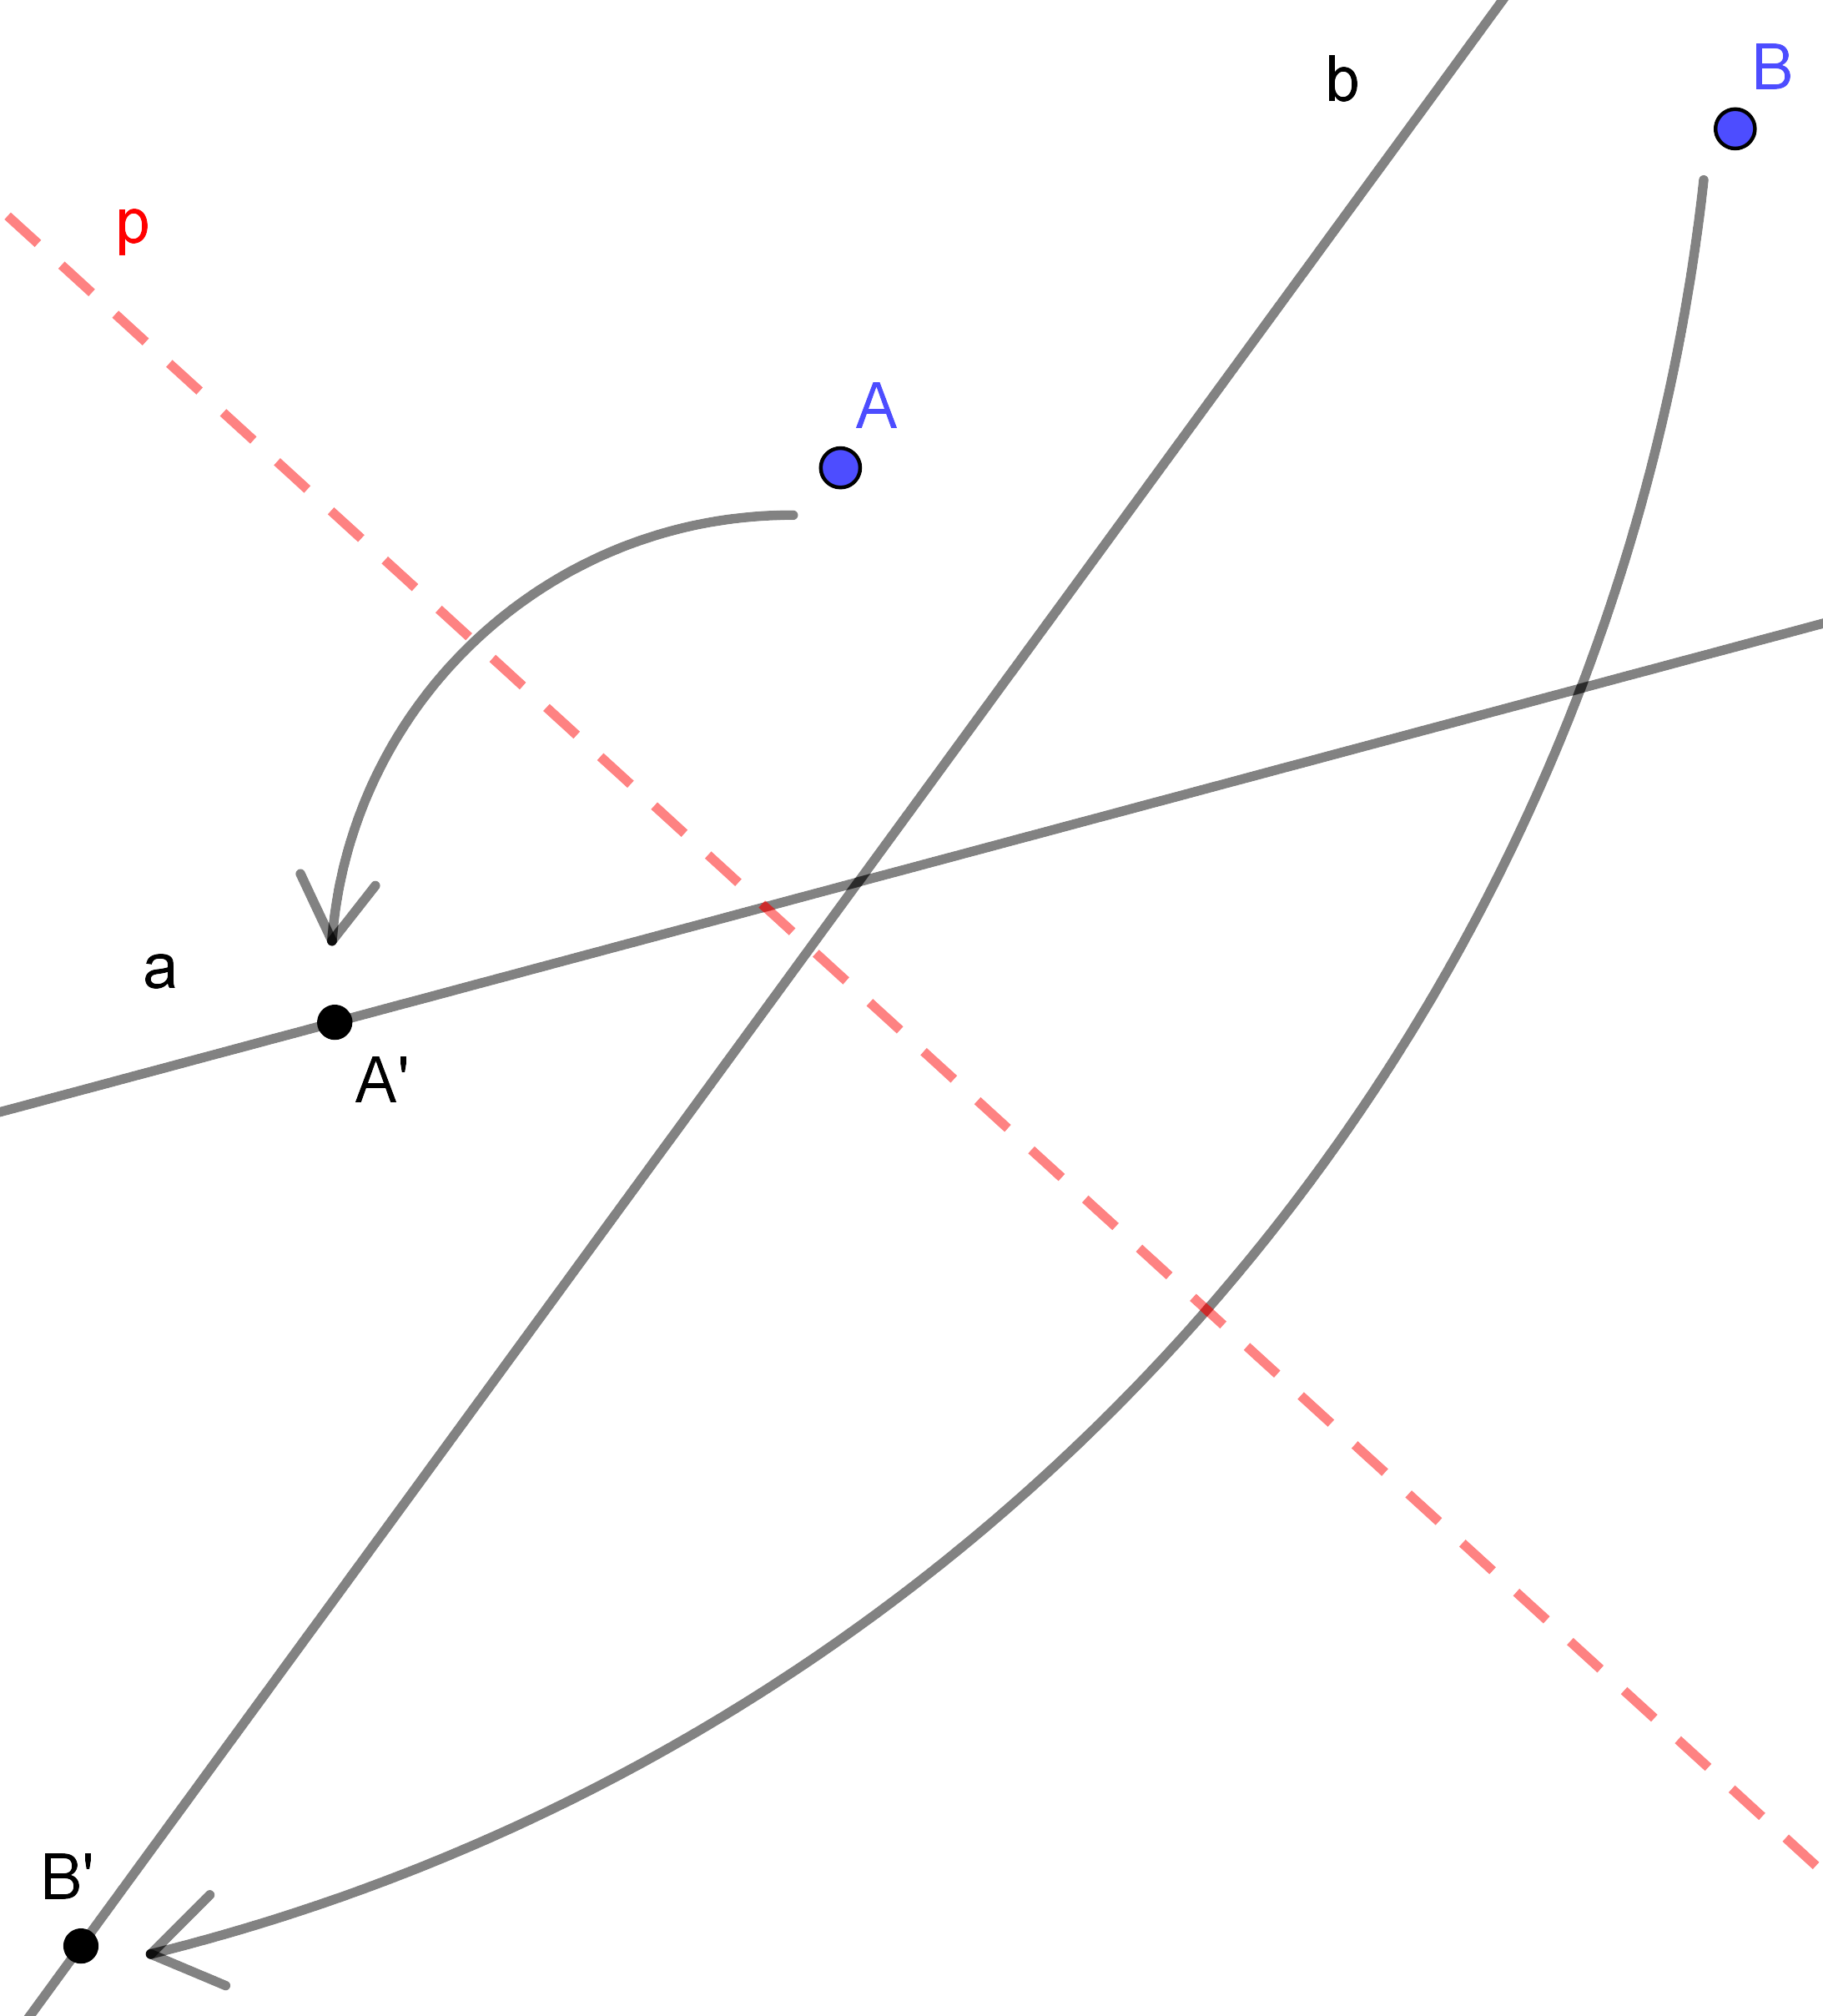
\includegraphics[width=0.45\textwidth]{images/origami_aksiomi/O6b.png}
    \caption[Aksiom~\ref{aks:O6}]{Aksiom~\ref{aks:O6} (primer dveh pregibov od najmanj treh možnih).}
    \label{fig:O6}
\end{figure}


 Možnosti konstrukcije z neoznačenim ravnilom in šestilom nima le aksiom~\ref{aks:O6}. Zakaj? Eden od dokazov je preko rešitve starogrškega problema o trisekciji kota. V poglavju~\ref{pogl:starogrskiproblemi} bomo spoznali več postopkov, ki nam kot razdelijo na tri skladne dele, pri tem pa uporabimo pregib iz aksioma~\ref{aks:O6}. Ker vemo, da trisekcija kota z evklidskim orodjem ni mogoča (algebraični dokaz \textcolor{red}{DEJ TU EN VIR ZA DOKAZ}), tudi konstrukcija šestega aksioma s tem orodjem ne obstaja.

\opomba{Opazimo, da je aksiom~\ref{aks:O5} poseben primer aksioma~\ref{aks:O6}, ko ena izmed točk že leži na premici, in bi ga v resnici lahko iz pravil izpustili. Vendar ga ohranimo ravno zaradi povezave prvih petih aksiomov z evklidskimi konstrukcijami.}
